\documentclass[article]{jss}

%% -- LaTeX packages and custom commands ---------------------------------------

%% recommended packages
\usepackage{orcidlink,thumbpdf,lmodern}

%% another package (only for this demo article)
\usepackage{framed}

\usepackage{amsmath}
\usepackage{cleveref}
\usepackage{subcaption}

%% new custom commands
\newcommand{\class}[1]{`\code{#1}'}
\newcommand{\fct}[1]{\code{#1()}}

\newcommand{\KM}{Kaplan--Meier} %chktex 8


%% -- Article metainformation (author, title, ...) -----------------------------

%% - \author{} with primary affiliation (and optionally ORCID link)
%% - \Plainauthor{} without affiliations
%% - Separate authors by \And or \AND (in \author) or by comma (in \Plainauthor).
%% - \AND starts a new line, \And does not.
\author{Jeffrey Roskes~\orcidlink{0000-0001-8761-0490}\\Johns Hopkins University} % chktex 8
\Plainauthor{Jeffrey Roskes}

%% - \title{} in title case
%% - \Plaintitle{} without LaTeX markup (if any)
%% - \Shorttitle{} with LaTeX markup (if any), used as running title
\title{\pkg{KoMbine}: Propagating Statistical and Systematic Errors to \KM{} Curves}
\Plaintitle{KoMbine: Propagating Statistical and Systematic Errors to \KM{} Curves}
\Shorttitle{\pkg{KoMbine}: Propagating Errors to \KM{} Curves}

%% - \Abstract{} almost as usual
\Abstract{
  \KM{} curves are widely used in medical research to evaluate the performance of biomarkers and predict patient outcomes. These curves are often shown without error bands, and even when error bands are provided, they typically only account for the statistical uncertainty resulting from the finite number of patients in the study. In reality, other sources of uncertainty affect the measurements as well. As datasets grow, the patient-wise statistical uncertainty no longer dominates the overall uncertainty, and other uncertainties are increasingly important to model. The \pkg{KoMbine} package, developed based on procedures used in particle physics, provides the first method to propagate both statistical and systematic uncertainties through the \KM{} curve estimation processes.
}

%% - \Keywords{} with LaTeX markup, at least one required
%% - \Plainkeywords{} without LaTeX markup (if necessary)
%% - Should be comma-separated and in sentence case.
\Keywords{kaplan--meier curve, uncertainty}
\Plainkeywords{kaplan-meier curve, uncertainty}

%% - \Address{} of at least one author
%% - May contain multiple affiliations for each author
%%   (in extra lines, separated by \emph{and}\\).
%% - May contain multiple authors for the same affiliation
%%   (in the same first line, separated by comma).
\Address{
  Jeffrey Roskes\\
  Institute for Data Intensive Engineering and Science\\
  \emph{and}\\
  Department of Physics and Astronomy\\
  Johns Hopkins University\\
  3400 N. Charles St\\
  Baltimore, MD 21218\\
  E-mail: \email{jroskes1@jhu.edu}
}

\begin{document}


%% -- Introduction -------------------------------------------------------------

%% - In principle "as usual".
%% - But should typically have some discussion of both _software_ and _methods_.
%% - Use \proglang{}, \pkg{}, and \code{} markup throughout the manuscript.
%% - If such markup is in (sub)section titles, a plain text version has to be
%%   added as well.
%% - All software mentioned should be properly \cite-d.
%% - All abbreviations should be introduced.
%% - Unless the expansions of abbreviations are proper names (like "Journal
%%   of Statistical Software" above) they should be in sentence case (like
%%   "generalized linear models" below).

\section{Introduction}\label{sec:intro}

\KM{} curves are widely used in medical research to predict patient outcomes by giving the survival probability as a function of time. Typically, a \KM{} curve starts with a survival probability of \(1.0\) at time \(0\), which represents, for example, the time of treatment. The survival probability decreases as time progresses, representing patient deaths or other events of interest.

Sometimes, a patient drops out of the study without experiencing the event of interest; such a patient is said to have been ``censored.'' The patient is included in the \KM{} curve until the point of censoring. After the patient is censored, they are no longer considered ``at risk'' for the event of interest, and the future survival probability is calculated based on the remaining patients.

\KM{} curves are often shown without error bands. Various popular packages, such as \pkg{survival} \citep{survival-package} in \proglang{R} \citep{R} or \pkg{lifelines} \citep{lifelines} in \proglang{Python}, use Greenwood confidence intervals to provide error bands that account for the statistical uncertainty resulting from the finite number of patients in the study~\citep{GreenwoodNotes,Greenwood}. (To be more precise, \pkg{lifelines} uses the exponential Greenwood confidence intervals, while \pkg{survival} allows several different methods, all variations of Greenwood's.)

Other uncertainties can also affect the \KM{} curve. These will typically be patient-wise uncertainties, which \emph{move} the patient from one \KM{} curve to another. For example, a biomarker study might classify patients based on the density of a particular cell type. A \KM{} plot could be constructed with two curves, for patients with a high and low density of the cell type. However, the cell type is subject to Poisson noise as well as systematic errors in the measurement. Similar errors apply to \KM{} plots that stratify patients by gene expression levels or other continuous variables.

The techniques in this paper are based on the \pkg{Combine} package \citep{CAT-23-001}, which was developed by the CMS Collaboration in particle physics\@. \pkg{Combine}, built on the \pkg{RooFit} framework \citep{RooFit} and the \pkg{Minuit} optimizer \citep{minuit}, is used for high-precision measurements of particle properties, which must account for tens or even hundreds of systematic uncertainties, and was used for such high-profile measurements as the discovery of the Higgs boson \citep{HIG-12-028} and subsequent measurements of its properties.

The \pkg{KoMbine} package provides the first method to propagate these types of errors through the \KM{} curve estimation process. It handles the statistical uncertainty on the number of patients in a more precise way than the Greenwood confidence intervals and incorporates patient-wise uncertainties into the calculation. The statistical and patient-wise uncertainties can also be plotted separately, allowing the user to see which uncertainties dominate.

\section{Methodology}\label{sec:methodology}

\pkg{KoMbine} uses a log-likelihood function to compute the confidence interval for each point on the \KM{} curve. The log likelihood is a function of the survival probability \(S\) as well as other parameters. We maximize the likelihood over those other parameters to find the ``likelihood scan'' as a function of \(S\) alone. The points of maximum likelihood form the \KM{} curve, and the confidence intervals are determined by the points where the log likelihood is below a threshold.

\subsection{Notation}\label{sec:notation}

We denote the inclusion of patient \(j\) by \(a_j\), which is \(1\) if the patient is included and \(0\) if the patient is excluded. The numbers of patients who were at risk and who died at time \(t_i\) are:
\begin{align}
r_i &= \sum_{t_j \geq t_i} a_j, \\
d_i &= \sum_{\substack{t_j = t_i \\ \neg c_j}} a_j,
\end{align}
where \(c_j\) indicates whether the patient was censored or not. We will allow \(a_i\) to vary so that \(r_i\) and \(d_i\) may differ from their nominal values \(\hat{r}_i\) and \(\hat{d}_i\).

The survival probability at time \(t_n\) is given by the \KM{} formula:
\begin{equation}
S_n = \prod_{i=1}^{n} p_i^\text{survived}, \label{eq:km-survival}
\end{equation}
where \(p_i^\text{survived}\) is the probability that a patient who has survived until a given time point continues to live. The nominal probability is calculated from the observed survival probabilities:
\begin{equation}
\hat{S}_n = \prod_{i=1}^{n} \left(1 - \frac{\hat{d}_i}{\hat{r}_i}\right). \label{eq:km-nominal}
\end{equation}

For clarity, we will distinguish the two types of uncertainty: the statistical uncertainty from the finite number of patients (which we will call the ``binomial uncertainty'') and the patient-wise uncertainty.

\subsection{Binomial uncertainty}\label{sec:binomial-uncertainty}

The binomial contribution to the \KM{} curve is computed from the number of patients at risk and the number of patients who died at each time point:
\begin{equation}
\mathcal{L}_{\text{binomial}}(p_i^\text{survived}, a_i) = \prod_{i=1}^{n} \binom{r_i}{d_i} {\left(p_i^\text{died}\right)}^{d_i} {\left(p_i^\text{survived}\right)}^{r_i-d_i},
\end{equation}
where \(p_i^\text{died} = 1 - p_i^\text{survived}\). The negative log likelihood (NLL) is
\begin{equation}
-\log \mathcal{L}_{\text{binomial}}(p_i^\text{survived}, a_i) = -\left[\sum_{i=1}^{n} \left( \log\binom{r_i}{d_i} + d_i \log p_i^\text{died} + (r_i-d_i) \log p_i^\text{survived} \right)\right]. \label{eq:binomial-nll}
\end{equation}

We are not interested in the individual \(p_i^\text{survived}\) values, but rather the overall survival probability \(S_n\). We therefore use \cref{eq:km-survival} as a constraint when we minimize the NLL\@.

\subsection{Patient-wise uncertainty}\label{sec:patient-wise-uncertainty}

We now consider that the patients themselves may be subject to uncertainty. Some patients who were nominally included in the \KM{} curve may actually be excluded or vice versa.

The classic case when this happens is when dividing the patients into groups based on a continuous parameter, such as gene expression or the density of a certain cell type. The parameter measurement is subject to uncertainty, which must be considered when determining the overall uncertainty on the \KM{} curve. (This is in contrast to \KM{} curves based on discrete categories with no error, such as treatment vs.\ placebo, where patient-wise uncertainty likely does not enter.)

We first precompute the NLL penalty for each patient to be included in the \KM{} curve, which is negative if the patient is nominally included and positive if the patient is nominally excluded. The penalty depends on the functional form of the patient's parameter's probability density function, and it is calculated as the difference between the minimum NLL for the parameter to be within the range to be included in the curve and the minimum NLL for it to be outside the range.

\pkg{KoMbine} allows several possible probability distributions for the patient parameters, including a delta function, Poisson distribution, a Poisson distribution divided by a fixed area (to represent, for instance, a density of cells), and a ratio of two Poisson distributions. Any of these can be multiplied by systematic uncertainties following the log-normal distribution, a common choice used to represent multiplicative uncertainties.

For the purpose of the math here, all that is important is that the penalty is a fixed number per patient, which we call \(-\log \mathcal{L}_j^{\text{patient}}\). We compute the NLL as
\begin{equation}
-\log \mathcal{L}_{\text{patient}}(a_j) = -\sum_{j=1}^{m} a_j\log \mathcal{L}_j^{\text{patient}}. \label{eq:patient-nll}
\end{equation}

\subsection{Combining the uncertainties}\label{sec:combining-uncertainties}

The total NLL is the sum of the binomial NLL and the patient-wise NLL\@:
\begin{equation}
-\log \mathcal{L}_{\text{total}}(p_i^\text{survived}, a_j) = -\log \mathcal{L}_{\text{binomial}}(p_i^\text{survived}, a_j) - \log \mathcal{L}_{\text{patient}}(a_j). \label{eq:total-nll}
\end{equation}

We minimize the overall NLL (\ref{eq:total-nll}) over the \(p_i^\text{survived}\) and \(a_j\), with the constraint (\ref{eq:km-survival}). This is a mixed integer nonlinear programming (MINLP) problem.

\subsection{Isolating the binomial and patient-wise uncertainties}\label{sec:isolating-uncertainties}

Although the total uncertainty on the \KM{} curve includes both the binomial and the patient-wise uncertainty, it is instructive to look at them separately. Determining which uncertainty dominates can help to understand the next steps in the analysis: should we try to enroll more patients or should we improve the biomarker measurements?

\subsubsection{Binomial uncertainty}

To examine the binomial uncertainty, we can fix the parameters to their nominal values, fixing \(a_j=\hat{a}_j=1\) for the patients who are nominally included and \(0\) for those who are nominally excluded. These results are approximately equivalent to the Greenwood confidence intervals used in other packages. As will be illustrated in \cref{sec:compare-to-greenwood}, our method is somewhat more precise, but is also computationally slower.

\subsubsection{Patient-wise uncertainty}

Isolating the patient-wise uncertainty is somewhat nontrivial. We cannot allow the survival probabilities \(p_i^\text{survived}\) to vary freely, as we would need the binomial term to constrain them. Instead, we fix
\begin{equation}
p_i^\text{survived}(a_j) = 1 - \frac{d_i(a_j)}{r_i(a_j)}.
\end{equation}

With this definition, \(S\) can only take on certain fixed, discrete values. Furthermore, depending on the order that patients were censored or died, values of \(S\) that are close together may actually only be reachable by very different combinations of patients included in the analysis, with correspondingly different NLL values. A scatter plot of \(-\log\mathcal{L}\) as a function of \(S\) would be useless.

Instead, we use a continuous variable \(S'\). We calculate \(\hat{S}\) using the nominal values of the patient parameters, as in \cref{eq:km-nominal}. Then, for any value of \(S'\), we minimize the NLL over \(a_i\) with the constraint that \(S\) is at least as far from \(\hat{S}\) as \(S'\):
\begin{align}
S \ge S' & \text{ if } S' > \hat{S} \\
S \le S' & \text{ if } S' < \hat{S}
\end{align}
This gives an interpretable visualization of the patient-wise uncertainty: we obtain the NLL that the survival probability is at least as far from the nominal probability as \(S'\). By construction, \(-\log\mathcal{L}(S')\) has a single minimum (either a single point or, if some patients are exactly on the boundary, a flat region) at \(\hat{S}\) and increases as \(S'\) moves away in either direction.

\section{Implementation}

\pkg{KoMbine} is implemented in \proglang{Python} and uses \pkg{Gurobi} \citep{gurobi} to minimize the NLL for a given value of \(S\).

We first minimize \(-\log \mathcal{L}_{\text{total}}\) without the constraint on \(S\) (\ref{eq:km-survival}) to find the maximum likelihood estimate and the best value of \(S\)\@. \code{scipy.optimize.brentq} \citep{brentq,scipy} is then used to compute the confidence intervals, bounded by the points where the NLL equals a threshold value (1.0 for 68\% CL and 3.84 for 95\% CL).

For the patient-wise-only error, there is no need to minimize the NLL over \(S'\), as by construction it minimizes at \(S'=S_\text{nominal}\). To find the confidence intervals, we use a binary search that only looks at the possible discrete values of \(S\): intermediate values of \(S'\) cannot return anything different.

\section{Examples and discussion}

This section provides examples that illustrate interesting aspects of the \KM{} curve estimation.

\subsection%
[Best fit vs. nominal \KM{} curve]% chktex 12
{Best fit vs.\ nominal \KM{} curve}

Counter-intuitively, the best fit \KM{} curve does not necessarily coincide with the nominal \KM{} curve. An example is shown in \cref{fig:best-fit-vs-nominal}.

If only the binomial penalty is included, the survival NLL always minimizes at the nominal survival probability. Similarly, with only the patient-wise errors, the nominal survival probability is also always optimal. However, when both are included, the two may differ.

To understand this, imagine a case where 7 patients were at risk at a particular time point and 4 of them survived. An additional patient who survived is nominally excluded from the curve, but their parameter is so close to the boundary that they can be included with only a small NLL penalty of \(0.01\)\@. \Cref{eq:binomial-nll} evaluates to \(-1.255\) for \(4\) patients surviving out of \(7\) with \(p_\text{survived}=4/7\), but to \(-1.267\) for \(5\) patients surviving out of \(8\) with \(p_\text{survived}=5/8\). This small difference in the binomial penalty outweighs the even smaller penalty for including the patient, and so the minimum NLL occurs at the best fit survival probability of \(5/8\).

This surprising result highlights the importance of the patient-wise uncertainties. If the NLL penalty for including the patient really is that small, then we cannot, with any confidence, assign the patient to one \KM{} curve or the other.

\begin{figure}
  \centering
  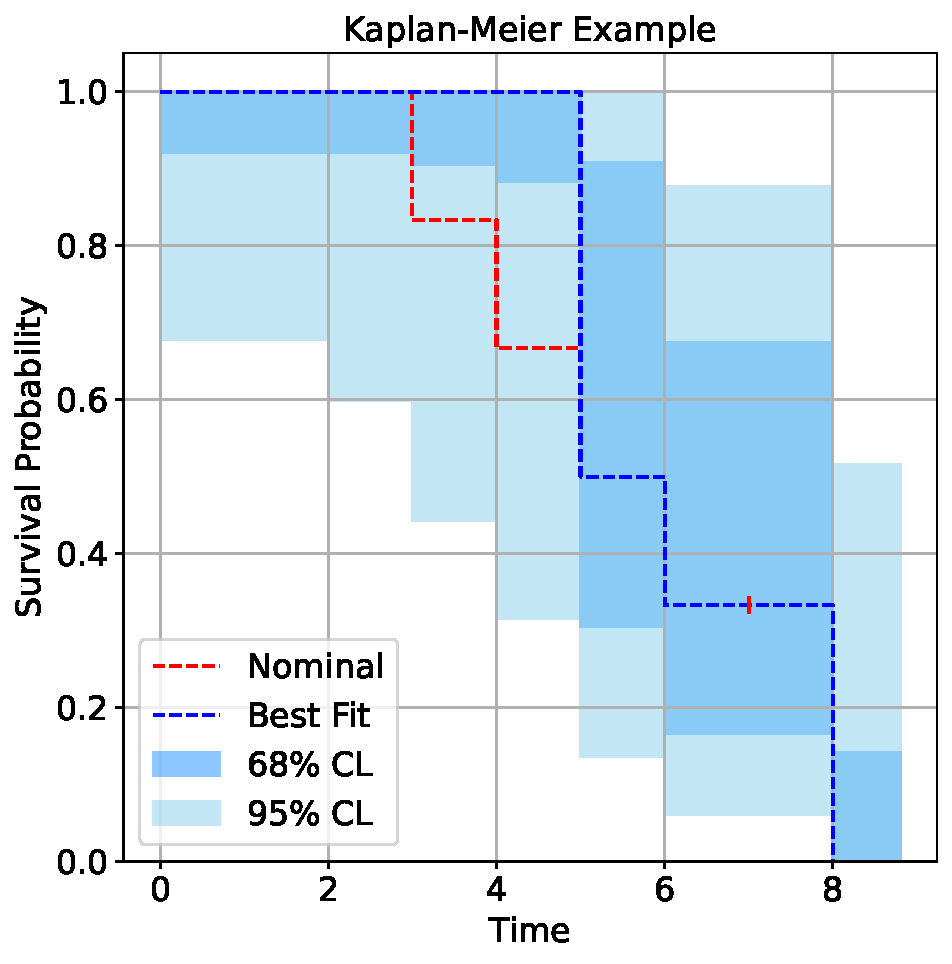
\includegraphics[width=0.5\textwidth]{km_example.pdf}
  \caption{\label{fig:best-fit-vs-nominal} An example \KM{} curve. The best fit (blue) does not coincide with the nominal curve (red). The error bands are shown as shaded blue areas.}
\end{figure}

\subsection{Lung cancer dataset}

This example is taken from \citet{DONUTS}, in which we analyzed pre-treatment biopsies from a cohort of patients with non-small-cell lung cancer (NSCLC) treated with anti-PD-1 immunotherapy. We identified CD8+FoxP3+ cells, which are associated with good outcomes but are extremely rare: a patient may have only one or two in their biopsy. We also developed a probabilistic biomarker, called DONUTS; DONUTS resemble the niche of the CD8+FoxP3+ cells but are much more abundant.

\Cref{fig:lung-dataset-cells} shows \KM{} curves for overall survival (OS) of patients with high and low densities of CD8+FoxP3+ cells. The patients with a high density of CD8+FoxP3+ cells have better outcomes, as expected, but the error bands are large due to the high Poisson uncertainty in the number of CD8+FoxP3+ cells. By contrast, \cref{fig:lung-dataset-donuts} shows the \KM{} curves for OS of patients with high and low densities of DONUTS\@. The error bands are smaller, as the DONUTS are much more abundant.

\Cref{fig:lung-dataset-cells-patient-wise,fig:lung-dataset-donuts-patient-wise,fig:lung-dataset-cells-binomial,fig:lung-dataset-donuts-binomial} show the same \KM{} curves with the uncertainties broken down into the patient-wise and binomial contributions. The binomial uncertainties have similar magnitude for the cells and for the DONUTS, as both have similar sample sizes in the high and low categories. The patient-wise uncertainties, on the other hand, are comparable to the binomial errors for the cells but almost zero for the DONUTS\@.

It should be noted that this is a fairly small cohort of only 25 patients. In a larger-scale study, the binomial uncertainties would be smaller and the difference in patient-wise uncertainties would be even more pronounced.

\begin{figure}[p]
  \newcommand{\spacebetweenrows}{1em}
  \newcommand{\figwidth}{0.36\textwidth}
  \centering
  \begin{subfigure}[t]{\figwidth}
    \centering
    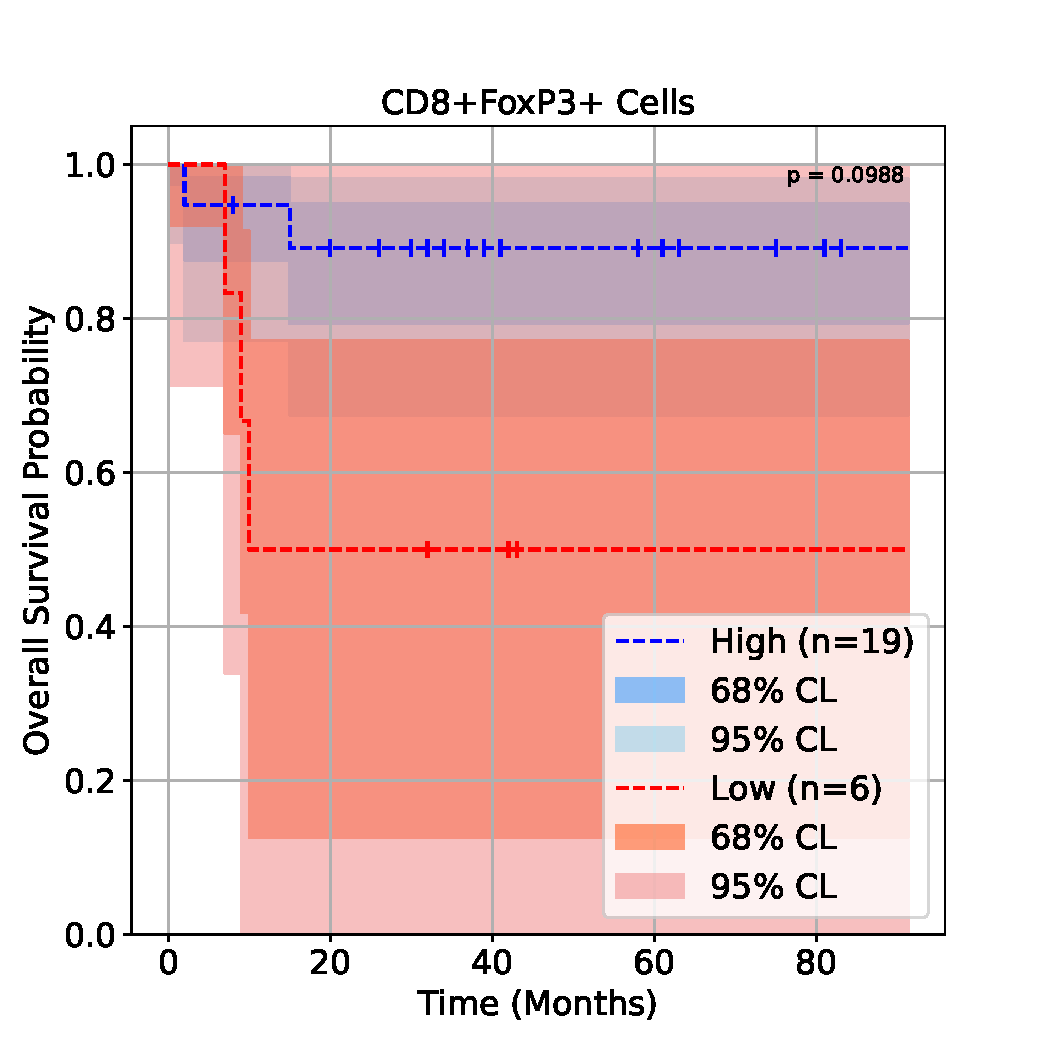
\includegraphics[width=\linewidth]{lung_cells_km_OS.pdf}
    \caption{\label{fig:lung-dataset-cells}}
  \end{subfigure}
  \begin{subfigure}[t]{\figwidth}
    \centering
    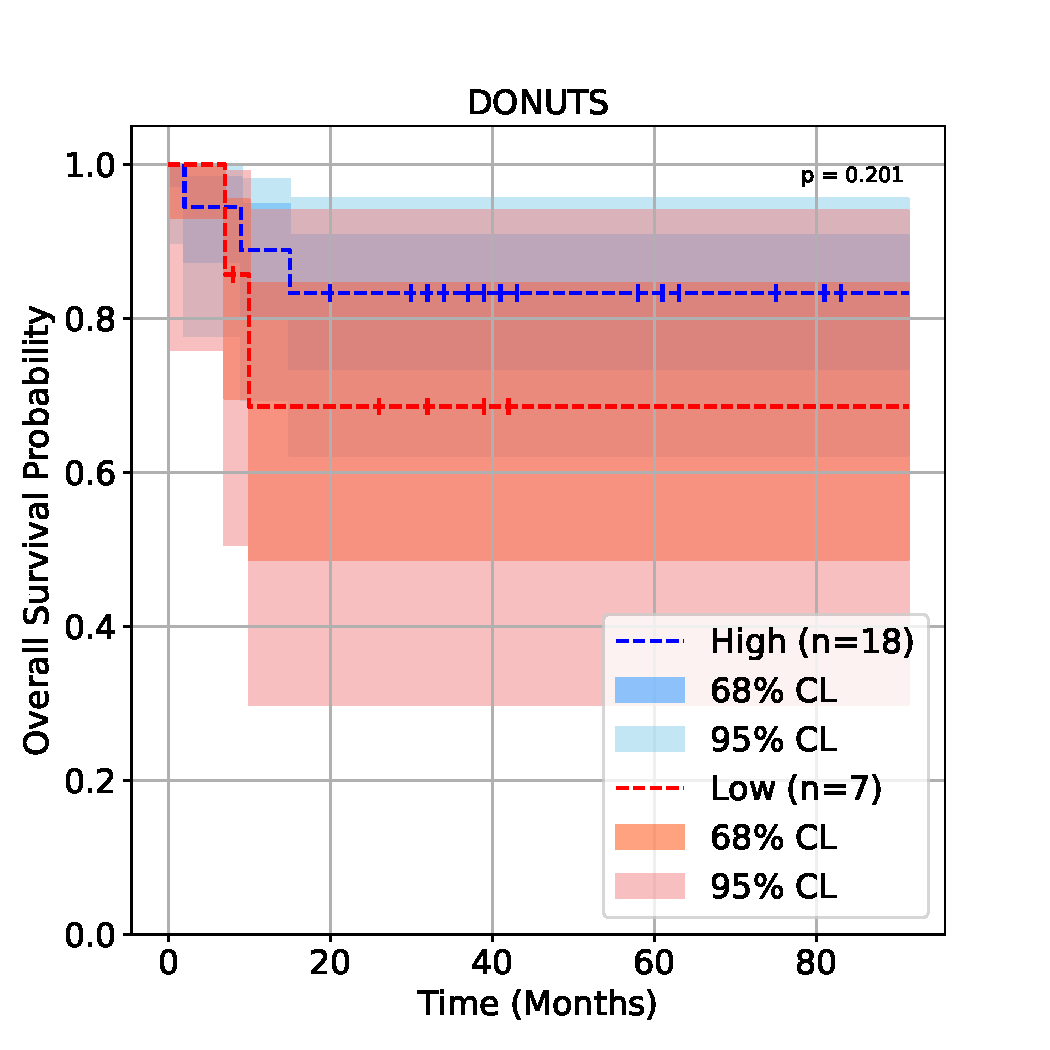
\includegraphics[width=\linewidth]{lung_donuts_km_OS.pdf}
    \caption{\label{fig:lung-dataset-donuts}}
  \end{subfigure} \\
  \vspace{\spacebetweenrows}
  \begin{subfigure}[t]{\figwidth}
    \centering
    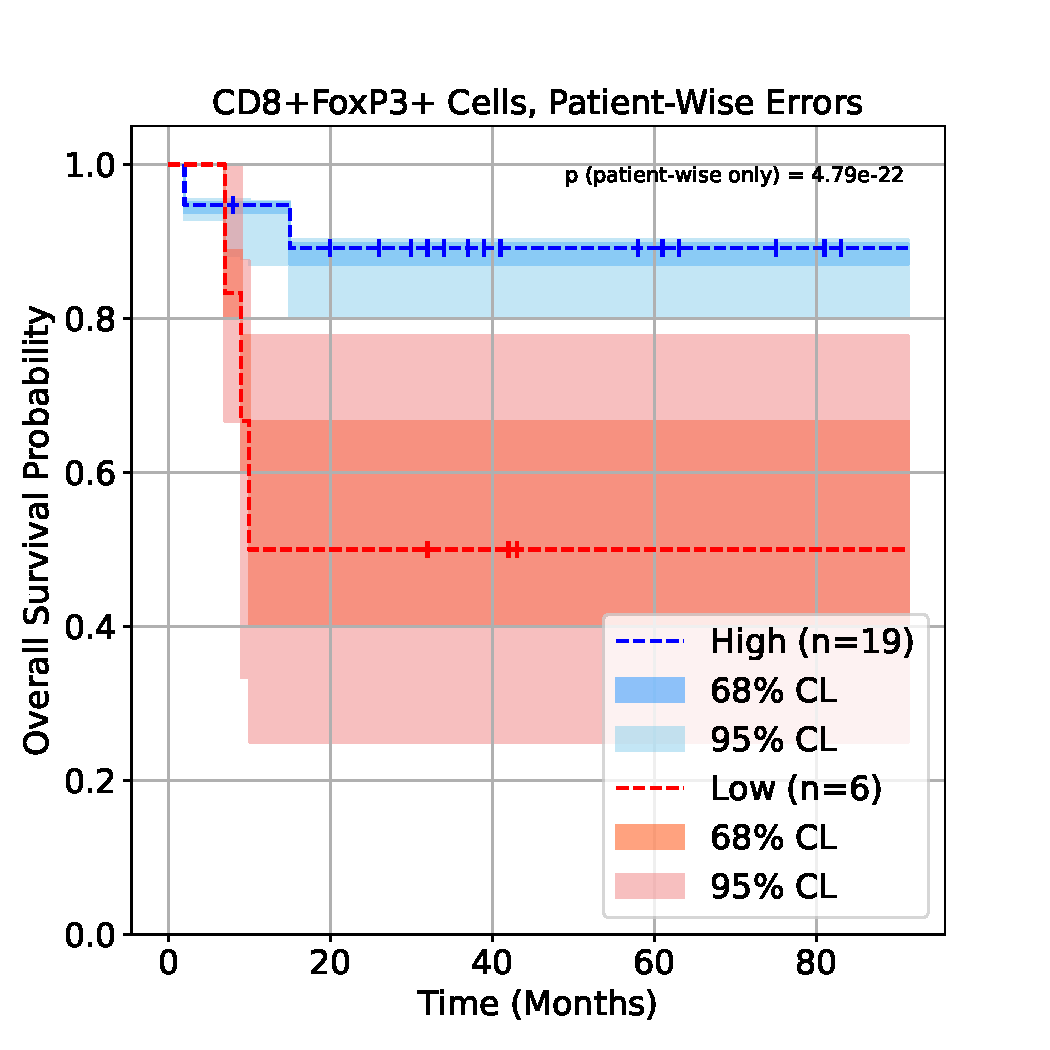
\includegraphics[width=\linewidth]{lung_cells_km_OS_patient_wise.pdf}
    \caption{\label{fig:lung-dataset-cells-patient-wise}}
  \end{subfigure}
  \begin{subfigure}[t]{\figwidth}
    \centering
    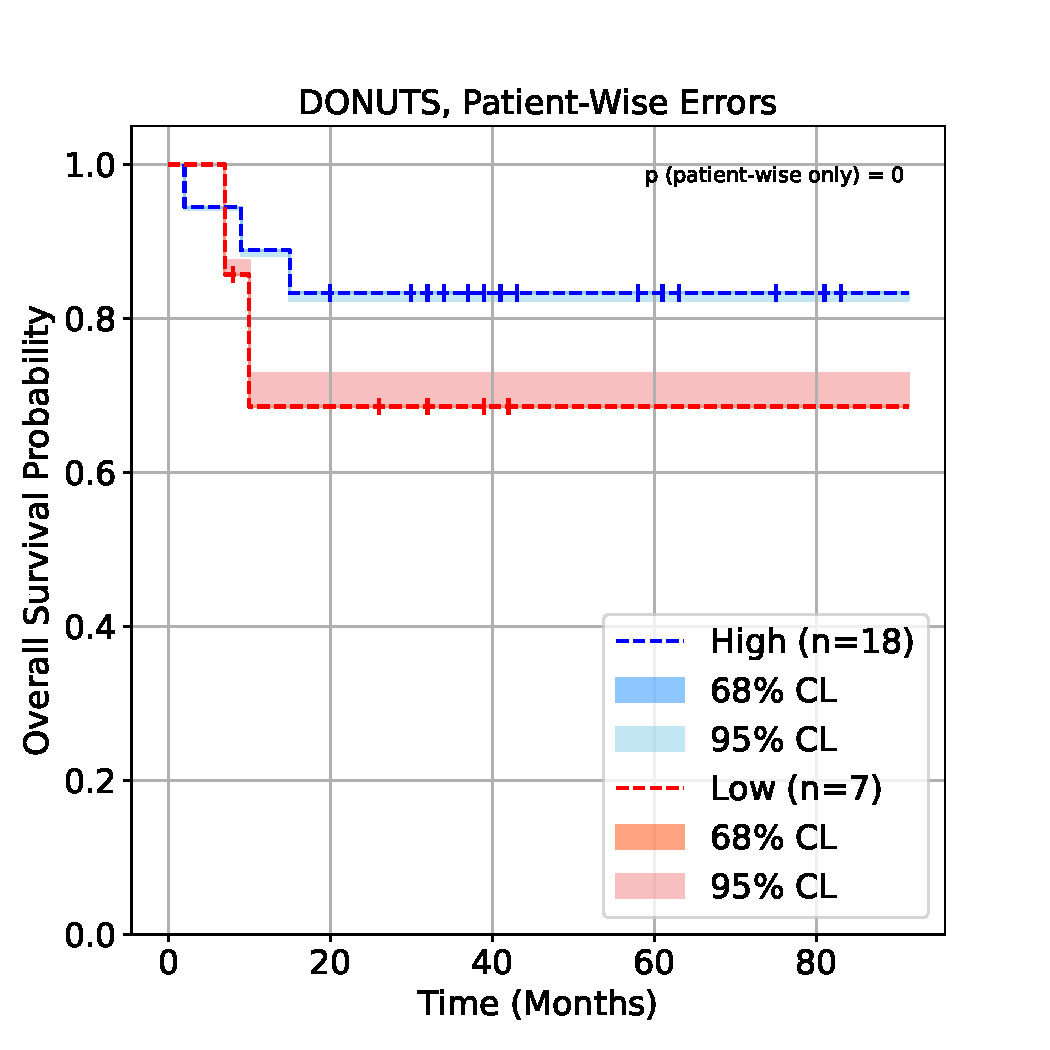
\includegraphics[width=\linewidth]{lung_donuts_km_OS_patient_wise.pdf}
    \caption{\label{fig:lung-dataset-donuts-patient-wise}}
  \end{subfigure} \\
  \vspace{\spacebetweenrows}
  \begin{subfigure}[t]{\figwidth}
    \centering
    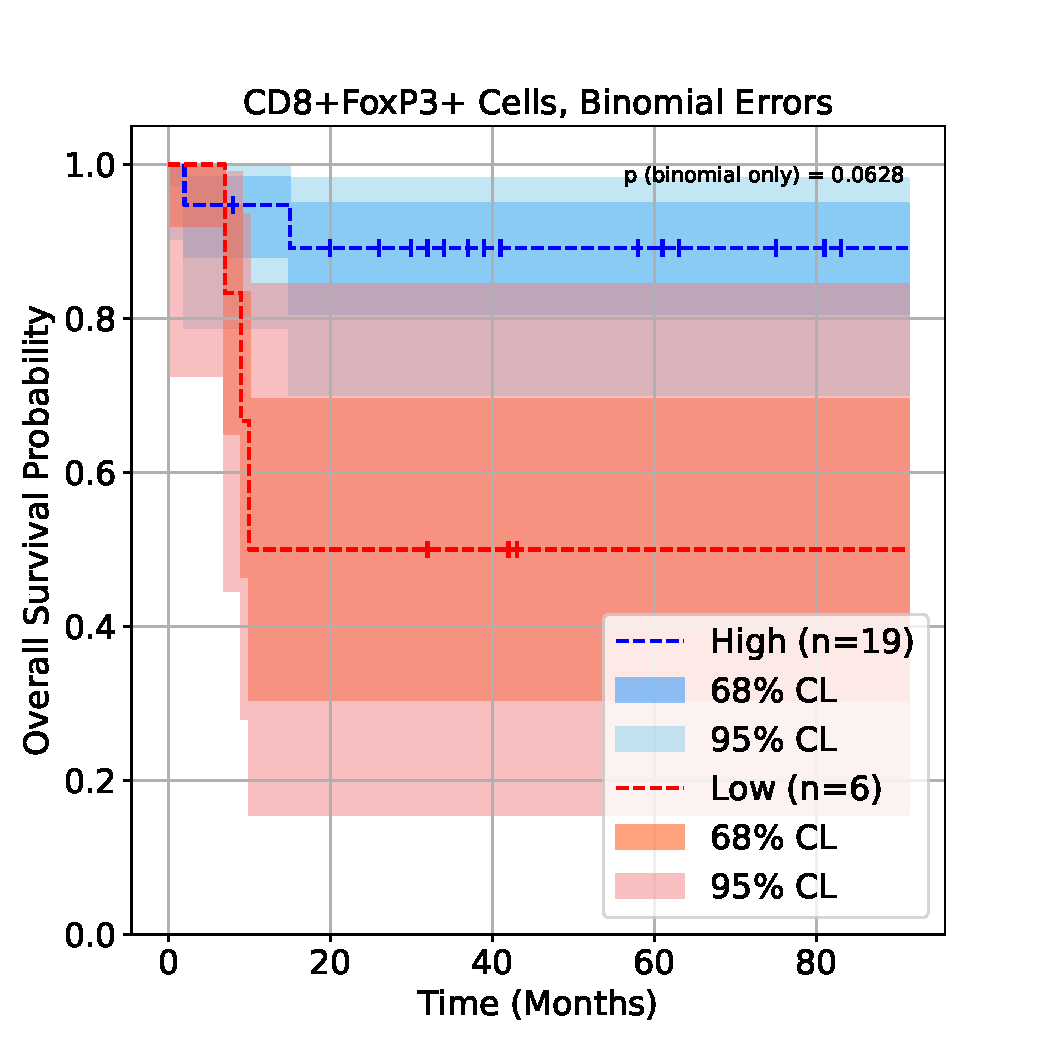
\includegraphics[width=\linewidth]{lung_cells_km_OS_binomial.pdf}
    \caption{\label{fig:lung-dataset-cells-binomial}}
  \end{subfigure}
  \begin{subfigure}[t]{\figwidth}
    \centering
    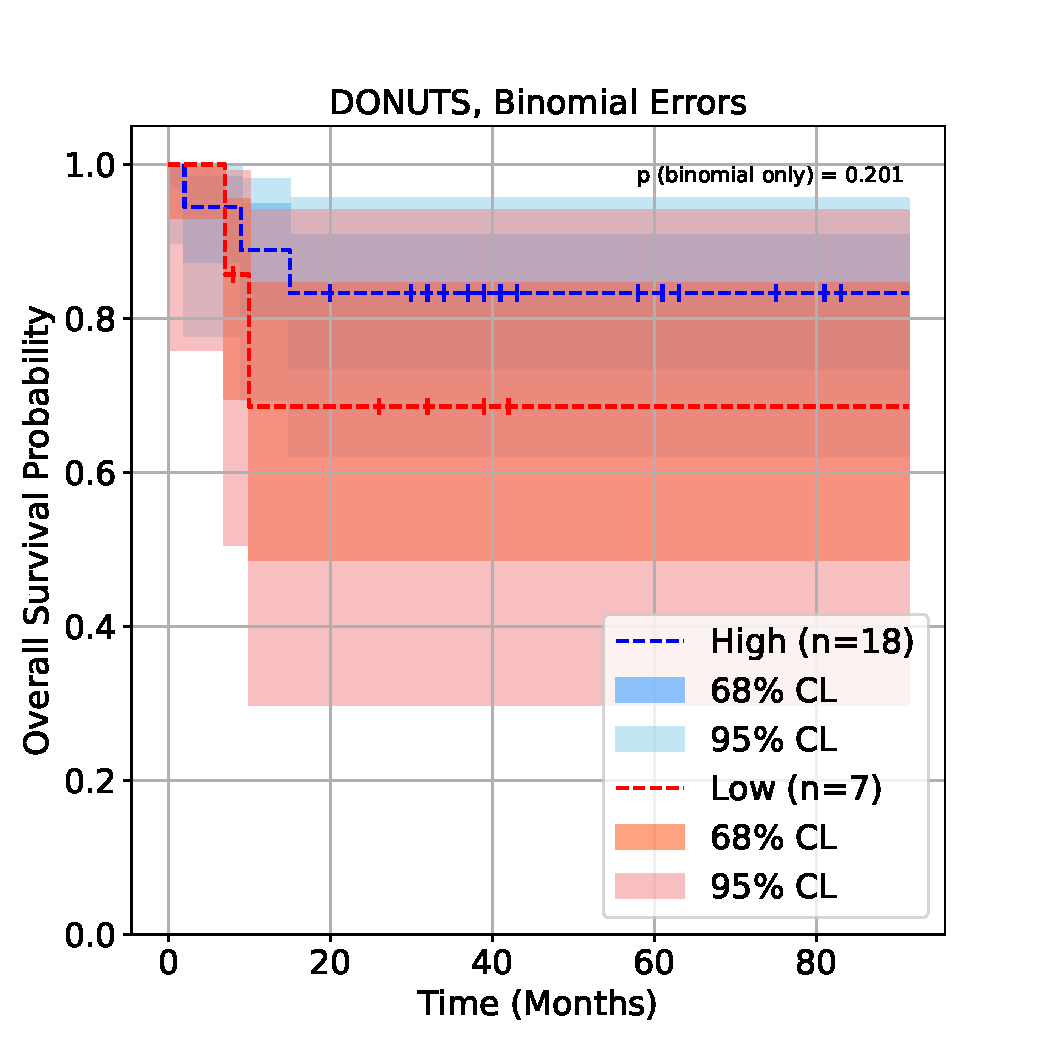
\includegraphics[width=\linewidth]{lung_donuts_km_OS_binomial.pdf}
    \caption{\label{fig:lung-dataset-donuts-binomial}}
  \end{subfigure}
  \caption{\label{fig:lung-dataset} \KM{} curves for the overall survival of patients with lung cancer, stratifying patients by their densities of either CD8+FoxP3+ cells (left) or DONUTS (right). The top row shows the full uncertainty, while the middle and bottom rows show the uncertainties broken down into patient-wise and binomial contributions, respectively.}
\end{figure}

\subsection{Comparison with Greenwood confidence intervals}\label{sec:compare-to-greenwood}

As mentioned earlier, most \KM{} curve packages provide confidence intervals using some variation of Greenwood's formula. At confidence level \(1-\alpha\), Greenwood's interval is given by
\begin{equation}
\label{eq:greenwood}
S(t)\in\hat{S}(t) \pm z_{\alpha/2} \sqrt{{\hat{S}(t)}^2{\sum_{i=1}^{n} \frac{d_i}{r_i(r_i-d_i)}}},
\end{equation}
where \(\hat{S}\) is the nominal value of the survival function, given by \cref{eq:km-nominal}. The exponential Greenwood interval is given by
\begin{equation}
\label{eq:exponential-greenwood}
\log{\left(-\log S(t)\right)} \in \log{\left(-\log \hat{S}(t)\right)} \pm z_{\alpha/2} \sqrt{\frac{1}{{\left(\log \hat{S}(t)\right)}^2} \sum_{i=1}^{n} \frac{d_i}{r_i(r_i-d_i)}}.
\end{equation}

\citet{GreenwoodNotes} gives the derivation of these formulas, which makes certain approximations: the ``delta-method'' approximation, which requires that the true and observed probabilities are close enough that \(\log\left(-\log S(t)\right)\) can be treated as approximately linear, and the approximation of the binomial distribution by a normal distribution. With large numbers of patients, these approximations hold, but their validity decreases for smaller cohort sizes.

\Cref{fig:compare-to-greenwood} shows \KM{} curves with the \pkg{KoMbine} confidence intervals and the Greenwood confidence intervals. The \pkg{KoMbine} are calculated with the binomial error only, to facilitate the comparison.

\begin{figure}
\centering
\begin{subfigure}[t]{0.49\textwidth}
  \centering
  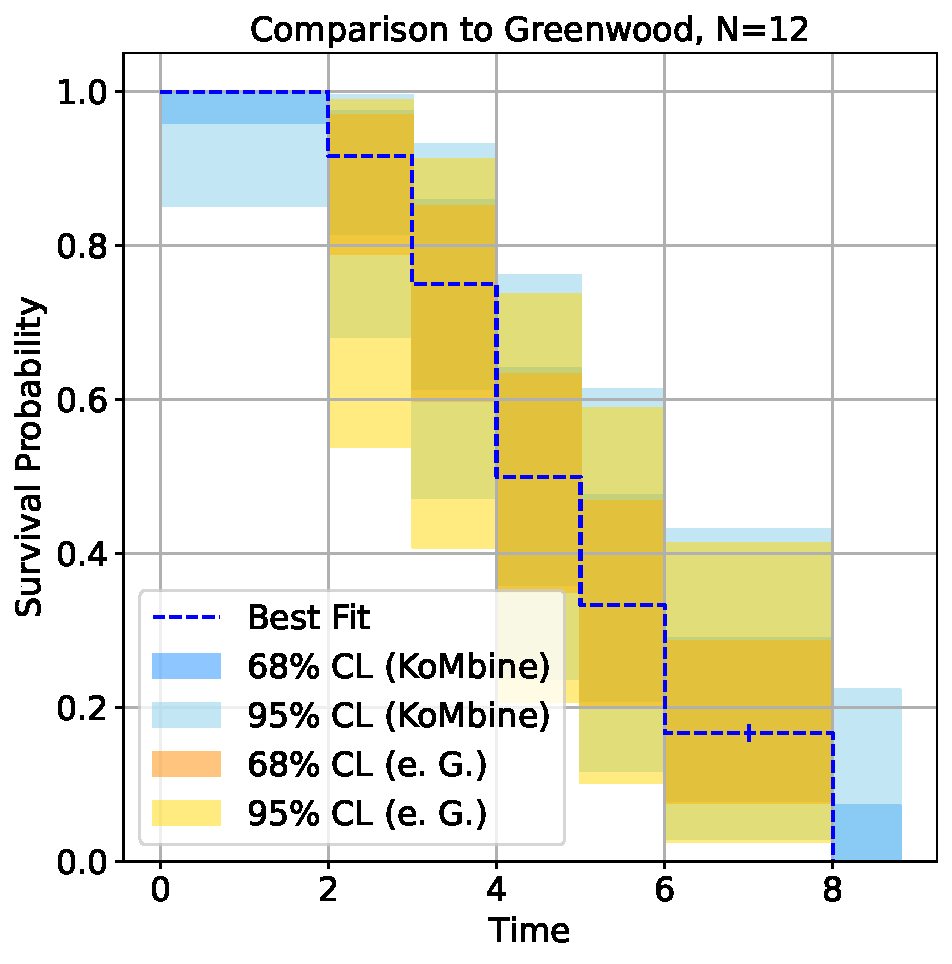
\includegraphics[width=\linewidth]{comparison_to_greenwood_small_n.pdf}
  \caption{\label{fig:compare-to-greenwood-small-n}}
\end{subfigure}
\begin{subfigure}[t]{0.49\textwidth}
  \centering
  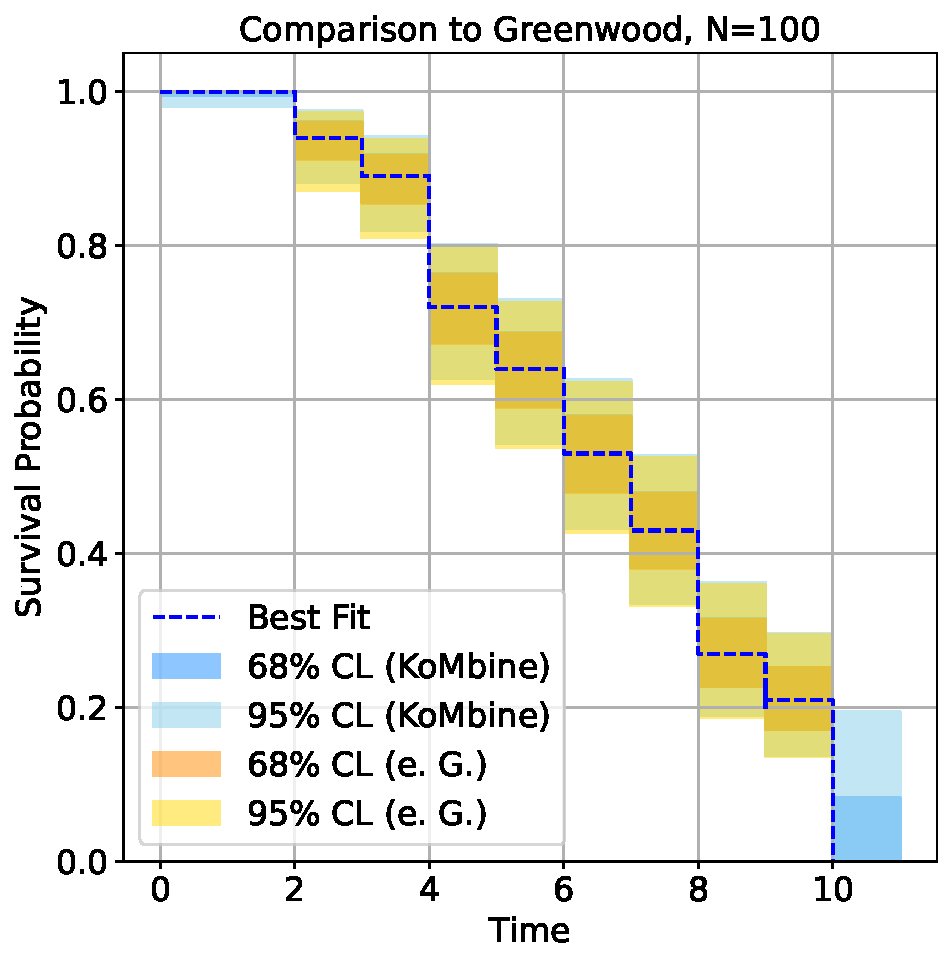
\includegraphics[width=\linewidth]{comparison_to_greenwood_large_n.pdf}
  \caption{\label{fig:compare-to-greenwood-large-n}}
\end{subfigure}
\caption{\label{fig:compare-to-greenwood} \KM{} curves with confidence intervals using only the binomial error, calculated using the exponential Greenwood (e. G.) formula from \cref{eq:exponential-greenwood} (gold) and the likelihood method from \pkg{KoMbine} (blue). The left panel shows a small cohort of 12 patients, while the right panel shows a larger cohort of 100 patients.}
\end{figure}

In \cref{fig:compare-to-greenwood-small-n}, only 12 patients are included in the \KM{} curve, and the exponential Greenwood confidence intervals are noticeably different from the \pkg{KoMbine} intervals. \Cref{fig:compare-to-greenwood-large-n} shows \KM{} curves with 100 patients, and the two confidence intervals are in agreement.

One striking difference in both cases is that the Greenwood method cannot calculate confidence intervals for the first or last time points, when the probabilities are \(1\) and \(0\). This is a fundamental limitation of the Greenwood method, which approximates the uncertainty on the \emph{true} binomial probability using the \emph{observed} numbers of patients who were at risk and who survived. If everyone survived or died, the binomial uncertainty is \(0\).

Our method, by contrast, calculates the binomial likelihood (and hence the uncertainty) using the \emph{true} survival probability, which we can do despite not knowing it in advance, because it is a parameter in the likelihood fit. This is the fundamental tradeoff of the likelihood method: we can be more precise, but the likelihood fit is more computationally intensive.

\section{Future work}

\subsection{Correlated uncertainties}

One important feature of \pkg{Combine} is uncertainties that are correlated between different channels. For example, uncertainties on the electron resolution affect, in different ways, the Higgs boson decay to four electrons or to two electrons and two muons.

Similarly, uncertainties resulting from batch effects in a biomarker assay will affect all patients in the same batch\@. \pkg{KoMbine} does not currently support this correlation. To implement it, \cref{eq:patient-nll} would need to be modified, as there would no longer be a fixed penalty per patient, but rather a penalty that depends on the other patients in the same batch. Furthermore, if there are multiple uncertainties correlated between different groups of patients, the penalty could depend on all patients at once.

The current \pkg{Gurobi} model would no longer work, as it requires precomputing \(\mathcal{L}_j^{\text{patient}}\). With \(N\) patients, we can easily precompute \(N\) values, but not \(2^N\). Instead, we would likely need to pass the uncertainty parameters \(\theta_k\) directly to the \pkg{Gurobi} model and let it compute \(a_j\left(\theta_k\right)\) and hence \(\mathcal{L}_{\text{patient}}\left(\theta_k\right)\) internally.

The increased number of continuous variables will probably require a rethinking of how the model is solved\@. \pkg{Gurobi} is not optimized for the types of complex nonlinear relationships that would be necessary here\@. \pkg{Minuit}, which forms the backbone for \pkg{Combine}, \emph{is} optimized for many continuous nuisance variables, but cannot handle indicator variables such as our \(a_j\), which are fundamental to the logic of \pkg{KoMbine}. Combining the strengths of both will be an interesting and nontrivial challenge.

\subsection{More advanced survival functionality}

The \pkg{lifelines} package provides support for other types of survival analysis, such as parameteric survival models, left and interval censoring, and other types of visualizations, such as cumulative hazard plots\@. \pkg{KoMbine} currently only supports the basic \KM{} curve, including right censoring, but similar statistical methods could be used to incorporate these other features.

\subsection{ROC curves}

Receiver operating characteristic (ROC) curves are also commonly used to evaluate biomarkers and predict patient outcomes. Similar statistical methods are necessary to propagate uncertainties through the ROC curve estimation process.

Some preliminary work, called \pkg{ROC Picker}, is available in the \pkg{KoMbine} package, but it is not yet fully functional. Crucially, it can handle either binomial or patient-wise uncertainties, but not both at the same time. ROC curve estimation is more complex because the uncertainties are correlated across all points in the curve, and the metrics typically used, such as the area under the curve (AUC), are nontrivial functions of the entire curve.

\section{Conclusion}

\pkg{KoMbine} provides a new method to propagate statistical and systematic uncertainties through the \KM{} curve estimation process. The handling of the binomial uncertainty is more precise than the Greenwood confidence intervals used in other packages, and the patient-wise uncertainties are implemented for the first time.

This package will enable uncertainty estimates on \KM{} curves to take \emph{all} sources of uncertainty into account, facilitating more robust and reproducible biomarker studies. Furthermore, by allowing the user to plot the different uncertainties separately, it will help researchers understand how to improve the analysis, furthering the development of the next generation of biomarkers.

\section*{Computational details}

The results in this paper were obtained using \proglang{Python}~3.11.13 with \pkg{numpy}~2.3.2, \pkg{scipy}~1.16.1, and \pkg{gurobipy}~12.0.3, as well as \pkg{Gurobi}~10.0.3. All \proglang{Python} packages can be installed using \pkg{pip} or \pkg{conda}.

\pkg{Gurobi} can be downloaded from \url{https://www.gurobi.com/}. Although it requires a license, free licenses are available for academic use.

\section*{Acknowledgments}

I would like to thank my AstroPath colleagues, in particular my mentors, Drs.~Alex Szalay and Janis Taube, for their support on this project. I would also like to acknowledge editing support by Ben Cohen, provided by the Office of the Vice Provost for Research at Johns Hopkins University.

This research was supported by the Mark Foundation for Cancer Research.

%% -- Bibliography -------------------------------------------------------------
%% - References need to be provided in a .bib BibTeX database.
%% - All references should be made with \cite, \citet, \citep, \citealp etc.
%%   (and never hard-coded). See the FAQ for details.
%% - JSS-specific markup (\proglang, \pkg, \code) should be used in the .bib.
%% - Titles in the .bib should be in title case.
%% - DOIs should be included where available.

\bibliography{08_kaplan_meier_paper}


%% -- Appendix (if any) --------------------------------------------------------
%% - After the bibliography with page break.
%% - With proper section titles and _not_ just "Appendix".

\newpage

\begin{appendix}

\section{Datacard format}\label{app:datacard}

The inputs to \pkg{KoMbine} are provided in a datacard format, similar to the one used in \pkg{Combine} \citep{CAT-23-001}. The datacard is a text file with the following format:
\begin{verbatim}
# Datacard for KoMbine
# This is a comment line
observable_type fixed
------------
# List of patients
------------
survival_time 3   4   5   2   4   5   6   4   3   6   8   7
censored      0   0   0   0   0   0   0   0   0   0   0   1
observable    0.1 0.2 0.3 0.4 0.5 0.6 0.3 0.4 0.5 0.6 0.7 0.8
\end{verbatim}
\end{appendix}
Any line starting with \code{\#} is a comment and is ignored, as are lines of hyphens \code{------------}.

The first line is the header, which specifies the type of observable. In this case, the observable is fixed, which means that there are no patient-wise uncertainties. The \code{survival\_time} gives the length of time the patient was observed before being censored or dying, and the \code{censored} line indicates whether the patient was censored (1) or not (0).

The \code{observable} line gives the value of the observable for each patient. The format is similar for other \code{observable\_type}s. This datacard gives the same nominal \KM{} curve as the previous example, but the patient-wise uncertainties are modeled as a ratio of two Poisson distributions:
\begin{verbatim}
observable_type poisson_ratio
------------
# List of patients
------------
survival_time 3   4   5   2   4   5   6   4   3   6   8   7
censored      0   0   0   0   0   0   0   0   0   0   0   1
num           10  20  30  40  50  60  30  40  50  60  70  80
denom         100 100 100 100 100 100 100 100 100 100 100 100
\end{verbatim}

To create a \KM{} plot, you can run:
\begin{CodeInput}
kombine datacard.txt km_plot.pdf --parameter-min 0.45
\end{CodeInput}
This will create a \KM{} plot with the patients whose parameter is at least \(0.45\) included in the curve.

You can also create a \KM{} plot with two curves, for patients with a high and low value of the observable:
\begin{CodeInput}
kombine_twogroups datacard.txt --parameter-threshold 0.45
\end{CodeInput}

The \code{--include-binomial-only} and \code{--include-patient-wise-only} options will calculate error bands that only include the binomial or patient-wise uncertainties, respectively, as described in \cref{sec:isolating-uncertainties}. By default, the error bands will be drawn hatched, with the combined uncertainty also displayed on the plot. If that is too hard to see, you can disable the combined uncertainty with \code{--exclude-full-nll}.

Various additional command line arguments are available and are documented in \code{kombine --help} or \code{kombine_twogroups --help}.

\end{document}
